\documentclass{article}
\usepackage{graphicx} % Required for inserting images
\usepackage{amsfonts}
\usepackage{amsmath}
\usepackage{amsthm}
\title{MA-138}
\author{Haria}
\date{October 2025}

\begin{document}

\maketitle

\section{Lecture 1 - Sets}
\newtheorem{definition}{Definition}
\newtheorem{example}{Example}
\subsection{What are Sets}
\begin{definition}
A set is a collection of elements
\end{definition}
Commonly these are denoted by a listing of elements within braces. For example $\{1,2,3\}$ is the set containing 1, 2, and 3. Sometimes ellipses may be used inside the set
\begin{example}
    $\{0,1,2,3,\dots\}$ denotes the set of the natural numbers $\mathbb{N}$
\end{example}
When ellipses are seen a natural continuation of elements is assumed in this case the rest of the natural numbers. Note here $\mathbb{N}$ contains $0$.

\begin{definition}
    If $x$ is and element of a set $X$ we nay write $x \in X$
\end{definition}
\begin{example}
    $1 \in \mathbb{N}$
\end{example}
We can also demonstrate the converse
\begin{example}
    $-1 \notin \mathbb{N}$
\end{example}
\subsection{Set Relations}
\subsubsection{Equality}
The first thing we want to be able to tell about pairs of sets is whether two are the same.
\begin{definition}
    Sets $X$ and $Y$ are equal if for every $x \in X$ we have $x \in Y$ and for every $y \in Y$ we have $y \in X$
\end{definition}
From this definition falls out two interesting things
\begin{itemize}
    \item Sets do not care about the order of their elements
    \item Sets do not care how many times their elements occur
\end{itemize}
This makes them fundamentally different from lists.
\begin{example}
    $\{1,2,3\} = \{2,2,3,1,1,3,3\}$
\end{example}
\subsubsection{Empty Set}
Before the next relation it is useful to introduce a special set known as the empty set.
\begin{definition}
    There exists a set $\emptyset$ such that there does not exist an $x \in \emptyset$ called the empty set
\end{definition}
An interesting result is given two empty sets $\emptyset_{1}$ and $\emptyset_{2}$ these two are always equal. This is because any element in the first is necessarily in the second and vice versa as their are no elements in either. This tells us that there is only one empty set.

\subsubsection{Numeric Sets}
Another useful set to know is as follows before the next relation
\begin{definition}
    The set denoted $\mathbb{[}n\mathbb{]} = \{0,1,2,\dots n-1\}$
\end{definition}
This is the set of all the natural numbers less than $n$ and is non-standard notation. 
\subsubsection{Subsets}
\begin{definition}
    We can say a set $X$ is a subset of a set $Y$ if for every $x \in X$ we also know that $x \in Y$ this is denoted $X \subseteq Y$
\end{definition}
\begin{example}
    $\{0,1\} \subseteq \{0,1,2\}$
\end{example}
\begin{example}
    $[n] \subseteq [n+1]$
\end{example}

From here we can derive the fact that if $X \subseteq Y$ and $Y \subseteq X$ we can say $X = Y$. Each direction of the subset satisfies half the condition for equality so having both directions of the subset we can claim equality. this is similar to how when $x \le y$ and $y \le x$ we know that $x = y$.

For every set $X$ we can also say two things
\begin{enumerate}
    \item $\emptyset \subseteq X$
    \item $X \subseteq X$
\end{enumerate}
Which is also similar to what we can say for $\le$
\subsection{Set Function}
\subsection{Power Set}
Every set can have many power sets so it is useful to be able to easily reference this collection of subsets
\begin{definition}
    For a set $X$ let $\mathcal{P}(X)$ denote its power set such that $x \in \mathcal{P}(X)$ if and only if $x \subseteq X$
\end{definition}
\begin{example}
    $\mathcal{P}(\{1,2\}) = \{\emptyset,\{1\},\{2\},\{1,2\}\}$
\end{example}
\begin{example}
    $\mathcal{P}(\emptyset) = \{\emptyset\}$
\end{example}
It is important to remember that $\{\emptyset\}$ is a distinct set from $\emptyset$ as the first contains $\emptyset$ as an element $\emptyset \in \{\emptyset\}$ 
We also have a useful result that 
\[|\mathbb{P}([[n]])| = 2^n\]
As for each element in $[[n]]$ for each subset of $[[n]]$ it can either be in or out of the subset.
\section{Lecture 2 + 3 - Functions}
\subsection{Specification}
\begin{definition}
    \textbf{Specification} : Let $X$ be a set and $S(x)$ be a property for $x \in X$. We can form a set \[\{x \in X | S(X)\}\] This gives the subset of $X$ satisfying $S(x)$ for all $x$ in the subset
\end{definition}
An example of this is $\{k \in \mathbb{N} | k < n\}$ being the set of natural numbers less than $n$. This is the same as the set $[[n]]$ as defined earlier.

It is important to make sure you keep track of what set you are specifying against. For example the sets $\{k \in \mathbb{N} | x^2 - 1 = 0\}$ and $\{k \in \mathbb{Z} | x^2 - 1 = 0\}$ are different sets as the latter also contains $-1$. Its also important to remember you are taking a subset of a set in this invocation. Not doing so is unrestricted comprehension and leads to Russel's paradox.
\begin{figure}[h]
    \centering
    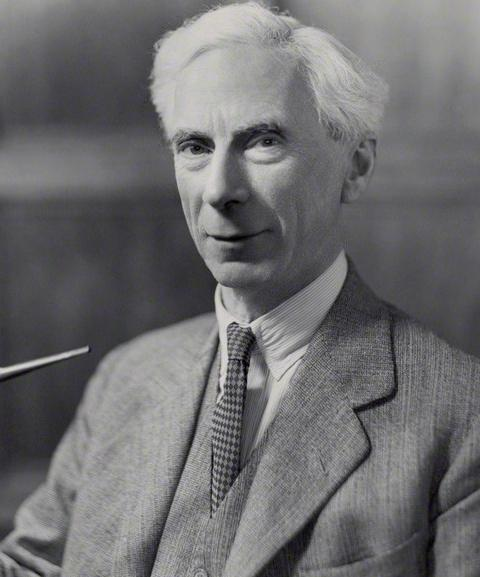
\includegraphics[width=0.3\linewidth]{russel.jpg}
    \caption{Russel angered by your use of unrestricted comprehension}
    \label{fig:placeholder}
\end{figure}
\\
\subsection{Functions}
\subsubsection{Basics}
Here we can start with a slightly informal definition of a function. 
\begin{definition}
    Let $X$ and $Y$ be sets. A function $f$ from $X$ to $Y$ (denoted $f:X \to Y$) contains three pieces of information
    \begin{enumerate}
        \item A domain $X$
        \item A codomain $Y$
        \item A rule mapping every in $x \in X$ to one $f(x) \in Y$
    \end{enumerate}
\end{definition}
Two examples of functions are given as $f_1:\mathbb{N} \to \mathbb{N}$ with $f_1(x) = x^2$ and another example is $f_2:\mathbb{N} \to \mathbb{Z}$ with $f_2(x) = x^2$. These both are are different functions as they have different codomains. Two functions are only equal if all three pieces of information agree.
\\
It is important to note that the rule portion of a function need not be given by a formula and can instead just tell you where each element goes. For example
$g : \{0,1\} \to \{2,3\}$ can have its rule expressed as $g(0) = 2$ and $g(1) = 2$. We can also get the useful property
\[|[[n]] \to [[m]]| = m^n\]
\\
If a function $f$ is $X \to X$ we say it is a function on $X$. A special function is the identity function on $X$ $id_{X}:X \to X$ given by rule $id_X(x) = x$
\subsubsection{Types of functions}
\begin{definition}
    A function $f:X \to Y$ is called injective if $f(x) = f(x') \Rightarrow x = x'$ for all $x,x' \in X$
\end{definition}
\begin{definition}
    A function $f:X \to Y$ is called surjective if for any $y \in Y$ there is an $x \in X$ such that $y = f(x)$
\end{definition}
And if a function satisfies both of these we can call it bijective.
\\
For finite sets we can say a lot of things about injections and surjections between them. For a pair of sets $X,Y$ if $|X| = |Y|$ then any injective function is surjective. this is due to the fact to be injective each element in the domain needs a separate element in the codomain. So their are as many elements in the image as the domain which is the same as the size of the codomain so every element in the codomain is hit. And for the reverse argument each element in the codomain binds a unique element in the domain which is every element in the domain. It cant bind 2 elements to one element in the codomain otherwise the image would not be the codomain and as such would not be surjective.
\\
We also get the fact we have no injections $f:[[n]] \to [[m]]$ if $m < n$ and no surjections $f:[[n]] \to [[m]]$ if $n<m$

\subsubsection{Cardinality}
\begin{definition}
    Given any sets $X$ and $Y$, $X$ and $Y$ have the same cardinality iff there exists a bijection $f:X \to Y$. This is denoted $|X| = |Y|$ 
\end{definition}
\begin{definition}
    For a finite set $X$ if there is a bijection $f:[[n]] \to X$ then we may say that $|X| = n$
\end{definition}
This makes sense for finite sets but has some interesting implications for infinite sets. Consider and $f:\mathbb{Z} \to \mathbb{N}$ defined as follows

    \[f(x) = \begin{cases}
        2x & \text{if } x \ge 0 \\
        -2x-1 & \text{if } x < 0
    \end{cases}\]
This function is a bijection between the two sets mapping even naturals to positives and odds to negatives. As such we have $|\mathbb{N}| = |\mathbb{Z}|$ despite $\mathbb{N} \subseteq \mathbb{Z}$. We can construct a similar argument between $\mathbb{N}$ and $\mathbb{Q}$ by use of \textbf{The Cantor Pairing Function} which constructs the bijection between pairs of natural numbers and naturals which gets you 99\% of the way to a bijection and infact shows that $|\mathbb{N}| \ge |\mathbb{Q}|$ as there are multiple pairs of naturals that can give a single rational number.
\\
This is however not possible between $\mathbb{R}$ and $\mathbb{N}$. It can be shown there is no such bijection. this is done using Cantor's diagonalization argument to prove that there is no surjection. 
\begin{proof}
    Assume that theres is a surjection $f:\mathbb{N}\to \mathbb{R}$ This would allow us to list elements of $\mathbb{R}$ on the output. Here we will represent elements of $\mathbb{R}$ in binary expansions
    \begin{align*}
        f(1) &= 0.010110101111\dots \\
        f(2) &= 0.101100110001\dots \\
        f(\cdots) &= \cdots \\
    \end{align*}
    Now we con construct a new number $x$. We make x by making the $n$th digit of $x$ the opposite of the $n$th digit of $f(n)$. Now the question is : is $x$ on our list. If $x$ is in the image of $f$ then there is some $k$ such that $f(k) = x$ but this means that $x$ will differ from $f(k)$ in the $k$th digit so $x$ cannot be $f(k)$ so $x$ cannot be in the image so $f$ cannot be a surjection
\end{proof}
\end{document}
